\chapter{Levantamento bibliográfico}
\section{Introdução ao capítulo}


\section{Padrão de arquitetura Model-View-Controller(MVC)}
    \par TODO: Quero colocar uma introdução do conceito de MVC menos aprofundada o que faço lá em baixo.
    
    \subsection{Contexto histórico}
    
        \par O padrão arquitetural Model-View-Controller (MVC) foi desenvolvido em 1978 por Trygve Reenskaug enquanto o mesmo trabalhava na Xerox PARC, com o objetivo de criar sistemas de informação que refletissem os modelos mentais dos usuários, promovendo uma interação intuitiva por meio de inspeção e edição de dados \cite[p.~1]{artigo:reenskaug:2003}. 
        
        \par Implementado inicialmente no ambiente Smalltalk, o MVC foi formalizado por Reenskaug em notas técnicas publicadas em maio e dezembro de 1979, que estabeleceram as bases do padrão \cite{artigo:reenskaug:1979}. Também é notável  que o Smalltalk foi o responsável pela criação do padrão MVC, que posteriormente se tornou amplamente adotado em sistemas orientados a objetos \cite{artigo:deacon:2009}.
        
        Ainda no contexto do Smalltalk-80, o MVC foi refinado para atender às demandas de interfaces gráficas dinâmicas, consolidando a separação de responsabilidades entre os componentes e introduzindo avanços como a distinção entre modelo de domínio (Md) e modelo de aplicação (Ma) \cite{artigo:deacon:2009}

        A validação e a demonstração de eficacia do padrão MVC, veio de um experimento no Xerox PARC, envolvendo um sistema de planejamento para uma fábrica de semicondutores, dessa forma 
        mostrando a sua aplicabilidade prática \cite{artigo:reenskaug:2003}. Com a evolução tecnológica, o MVC foi adaptado para interfaces mais complexas e inspirou frameworks modernos, como o ASP.NET MVC, que foi lançado em 2009 \cite{artigo:deacon:2009}.
        
    \subsection{Definindo conceitos}
        \par O MVC é um padrão arquitetural que separa a lógica do domínio (Model), a apresentação dos dados (View) e a interação do usuário (Controller), promovendo modularidade, reutilização e manutenção do sistema\cite{artigo:reenskaug:2003}.

        \par O MVC foi concebido para criar sistemas habitáveis, nos quais os usuários interagem com representações computacionais de objetos do mundo real, como recursos ou atividades, de forma natural \cite{artigo:reenskaug:2003}.

        \par O model é responsável por gerenciar os dados e a lógica do domínio, sem necessidade de dependência das interfaces, enquanto as Views exibem as informações e os Controllers processam as entradas do usuário \cite{artigo:deacon:2009}.

        \begin{figure}[H] % O [H] exige o uso do pacote float (veja abaixo)
            \centering
            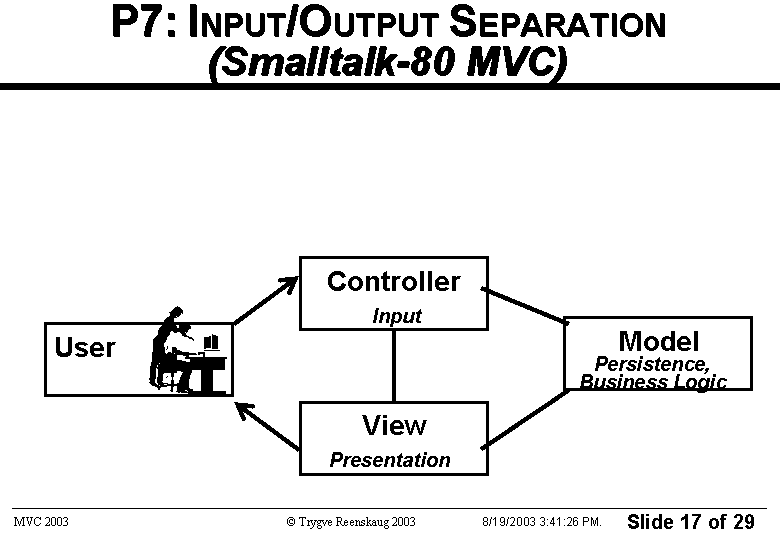
\includegraphics[width=0.8\textwidth]{figuras/figura_mvc_1.png}
            \caption{Modelo de colaboração UML da solução Smalltalk-80.}
            \label{fig:figura_mvc_1}
            \newcommand{\source}{Fonte: \cite{artigo:reenskaug:2003}}
        \end{figure}

        \subsubsection{Um model com multiplas views}
            \par O model representa a essência do domínio do problema, encapsulando os dados e a lógica de negócio sem qualquer conhecimento sobre as interfaces que o acessam. Essa independência permite que um único Model suporte múltiplas Views, que são as interfaces responsáveis por apresentar os dados ao usuário \cite{artigo:deacon:2009}.

            \par As views podem variar de acordo com a necessidade da aplicação que vai fazer uso do padrão, abrangendo interfaces gráficas (GUI), interfaces de linha de comando (CLI) ou até mesmo interfaces de programação (API) \cite{artigo:deacon:2009}.

            \par A separação entre o Model e as Views garante que as mudanças na interface não impactem a lógica da aplicação, facilitando a migração de sistemas legados, como aplicações bancárias que passaram de interfaces baseadas em caracteres para interfaces gráficas modernas \cite{artigo:deacon:2009}.
        
        \subsubsection{O modelo de domínio e modelo da aplicação}
            \par Um avanço significativo foi a distinção entre o modelo de domínio (Md), que encapsula a essência do problema, e o modelo de aplicação (Ma), que coordena as interações com as Views, clarificando as funções de cada componente \cite{artigo:deacon:2009}
            %% DA PRA APROFUNDAR MAIS AQUI NO ARTIGO EXPLICA

        \subsubsection{A comunicação da View para o Model}
            \par A comunicação entre esses componentes ocorre por meio de eventos, garantindo baixo acoplamento e alta flexibilidade \cite{artigo:deacon:2009}. 
            %% TODO: DA PRA APROFUNDAR MAIS AQUI NO ARTIGO EXPLICA
            
        \subsubsection{A comunicação do Model e Controller para a View}
            %% TODO: DA PRA APROFUNDAR MAIS AQUI NO ARTIGO EXPLICA

    
        \subsection{Padrão MVC no Smalltalk-80}

            \par Conforme já mostrado no presente trabalho o MVC tem sua origem no Smalltalk-80, tendo isso em vista podemos detalhar como funcionava a implementação inicial desse padrão trazendo bons pararelos para as implementações mais modernas desse padrão.
        
            \par O padrão MVC estabeleceu uma arquitetura inovadora para sistemas interativos \cite{artigo:reenskaug:2003}. No Smalltalk-80, o Model representava a base do sistema, encapsulando os dados e o comportamento essencial do domínio da aplicação \cite{artigo:reenskaug:2003}. A View assumia a responsabilidade pela apresentação visual dos dados contidos no Model, podendo existir múltiplas Views para um mesmo Model, como já mencionado anteriormente \cite{artigo:reenskaug:2003}. 
            
            \par O Controller funcionava como mediador entre as ações do usuário e o sistema, interpretando eventos de entrada e traduzindo-os em operações específicas \cite{artigo:reenskaug:2003}. Em componentes mais simples, como as barras de rolagem, os papéis de View e Controller frequentemente se fundiam em um único objeto \cite{artigo:reenskaug:2003}.

            \par Nesse mesmo contexto, o mecanismo de sincronização entre Model e View operava através do padrão Observer, onde modificações no Model automaticamente notificavam todas as Views registradas para o mesmo \cite{artigo:reenskaug:2003}. Com o objetivo de otimizar o desempenho da aplicação, implementavam-se técnicas como transações que agrupavam múltiplas alterações antes de propagá-las às Views \cite{artigo:reenskaug:2003}.
            
            \par Além disso, a arquitetura ainda previa o conceito de Tools, que coordenavam conjuntos de Editores (Views) para tarefas complexas, garantindo consistência na interface \cite{artigo:reenskaug:2003}. 
            
            \par Esta implementação do MVC no Smalltalk-80 serviu como base, definindo os princípios fundamentais de separação de preocupações que influenciaram profundamente o desenvolvimento de interfaces gráficas no futuro \cite{artigo:reenskaug:2003}
            
    
    \subsection{Padrão MVC na WEB}

        \par O padrão Model-View-Controller (MVC) foi adaptado para a web a partir do conceito original desenvolvido no ambiente Smalltalk e com o surgimento de frameworks web, como Apache Struts, o MVC foi reformulado para atender à arquitetura cliente-servidor, onde a view opera no navegador, fisicamente separada do model e controller hospedados no servidor \cite{inproceedings:grove:2011}. 
        
        \par Essa separação exigiu a introdução do padrão Front Controller, no qual um controlador central roteia requisições HTTP com base na URL solicitada e em configurações específicas, marcando a transição do MVC clássico para o contexto web \cite{inproceedings:grove:2011}.

        \par Frameworks web como o Ruby on Rails e ASP.NET MVC consolidaram o uso do MVC na web, adaptando-o para facilitar o desenvolvimento de aplicações dinâmicas. Em Rails, os ActionControllers gerenciam requisições, filtram parâmetros, orquestram transações no model e preparam dados para views, que são templates HTML com scripts Ruby embutidos \cite{inproceedings:grove:2011}.
        
        \par Da mesma forma, no framework ASP.NET MVC, controllers processam requisições, coordenam transações no model e ativam views dinâmicas definidas em arquivos ASP com scripts server-side \cite{inproceedings:grove:2011}. 

        \par Nessas duas implementações em frameworks diferentes, o controller assumiu um papel mais central, decidindo qual view exibir com base no resultado das ações, enquanto a view passou a incorporar comportamentos interativos no lado do cliente, como validação de entrada ou atualizações via JavaScript e Ajax, para melhorar a responsividade \cite{inproceedings:grove:2011}.

        \par O padrão MVC-Web, que emergiu dessas adaptações, reflete as particularidades do ambiente web. Diferentemente do MVC original, ele não utiliza o padrão Observer para notificar a view sobre mudanças no model. Em vez disso, o controller gerencia a propagação de atualizações e o fluxo da aplicação \cite{inproceedings:grove:2011}.
        
        \par O model, menos rigidamente definido, é composto por objetos instanciados sob demanda para lidar com lógica de negócios e transações, com o banco de dados servindo como componente persistente. A view, além de ter o papel de exibir dados, pode consultar o modelo diretamente e executar funções como validação de entrada, o que compromete a separação de responsabilidades, mas aumenta a eficiência \cite{inproceedings:grove:2011}. 
        
        \par Algumas tecnologias do lado do cliente como Ajax intensificaram essa tendência, tornando as fronteiras dos componentes do MVC mais fluidas, diferente da modularidade definida originalmente pelo padrão \cite{inproceedings:grove:2011}.

        \subsubsection{Componente Modelo}
        
            \par O \textbf{Modelo} (Model) é responsável por gerenciar o estado da aplicação e suas regras de negócio. Suas funcionalidades incluem:
        
            \begin{itemize}
                \item Persistência de dados: Armazenamento e recuperação de informações, seja em bancos de dados ou por meio de interfaces abstratas.
                \item Processamento de transações: Execução da lógica que altera o estado da aplicação (ex.: cálculos, atualizações).
                \item Integração com sistemas externos: Comunicação com APIs, serviços web ou sistemas legados.
                \item Resposta a consultas: Fornecimento de dados aos demais componentes (View e Controller) quando solicitado.
            \end{itemize}
        
        \subsubsection{Componente Visualização (View)}
            \par A \textbf{Visualização} (View) lida com a interface do usuário, focando na apresentação e interação. Suas atribuições são:
        
            \begin{itemize}
                \item Exibição de conteúdo: Renderização de dados obtidos do Modelo, como páginas HTML ou respostas JSON.
                \item Captura de interações: Disponibilização de formulários, botões e outros elementos de entrada.
                \item Comportamento dinâmico: Uso de tecnologias como JavaScript e Ajax para validação, autocompletar ou atualizações assíncronas — em alguns casos, sobrepondo-se a validações do Modelo.
            \end{itemize}
        
            \subsubsection{Componente Controlador (Controller)}
                \par O \textbf{Controlador} (Controller) atua como mediador, coordenando as requisições e o fluxo da aplicação. Suas tarefas principais são:
        
                \begin{itemize}
                    \item Front Controller: Receber e rotear requisições aos manipuladores corretos.
                    \item Validação e orquestração: Checar parâmetros (ex.: dados de formulários) e invocar métodos do Modelo para processá-los.
                    \item Gerenciamento de fluxo: Decidir qual View será exibida após o processamento (ex.: redirecionar após um login bem-sucedido).
                \end{itemize}
        
                \subsubsection{Interações entre Componentes}
                \par A comunicação entre os módulos segue um fluxo definido:
        
                \begin{itemize}
                    \item Model $\rightarrow$ View: A View consulta o Modelo para obter dados a serem exibidos (ex.: listagem de produtos).
                    \item Controller $\rightarrow$ Model: O Controller solicita ao Modelo a execução de operações (ex.: salvar um registro no banco de dados).
                    \item Controller $\rightarrow$ View: O Controller seleciona a View apropriada e envia dados para renderização (ex.: exibir mensagens de erro).
                \end{itemize}
                
        \par Essa evolução do MVC na WEB responde às demandas de aplicações web mais modernas, que exigem maior interatividade e rapidez. No entanto, a incorporação de lógica de aplicação na view e no controller, como validação de dados ou manipulação de interface, pode dificultar a manutenção e a extensibilidade, já que dilui a separação clara de responsabilidades do MVC clássico \cite{inproceedings:grove:2011}.
        